\documentclass[1p]{elsarticle_modified}
%\bibliographystyle{elsarticle-num}

%\usepackage[colorlinks]{hyperref}
%\usepackage{abbrmath_seonhwa} %\Abb, \Ascr, \Acal ,\Abf, \Afrak
\usepackage{amsfonts}
\usepackage{amssymb}
\usepackage{amsmath}
\usepackage{amsthm}
\usepackage{scalefnt}
\usepackage{amsbsy}
\usepackage{kotex}
\usepackage{caption}
\usepackage{subfig}
\usepackage{color}
\usepackage{graphicx}
\usepackage{xcolor} %% white, black, red, green, blue, cyan, magenta, yellow
\usepackage{float}
\usepackage{setspace}
\usepackage{hyperref}

\usepackage{tikz}
\usetikzlibrary{arrows}

\usepackage{multirow}
\usepackage{array} % fixed length table
\usepackage{hhline}

%%%%%%%%%%%%%%%%%%%%%
\makeatletter
\renewcommand*\env@matrix[1][\arraystretch]{%
	\edef\arraystretch{#1}%
	\hskip -\arraycolsep
	\let\@ifnextchar\new@ifnextchar
	\array{*\c@MaxMatrixCols c}}
\makeatother %https://tex.stackexchange.com/questions/14071/how-can-i-increase-the-line-spacing-in-a-matrix
%%%%%%%%%%%%%%%

\usepackage[normalem]{ulem}

\newcommand{\msout}[1]{\ifmmode\text{\sout{\ensuremath{#1}}}\else\sout{#1}\fi}
%SOURCE: \msout is \stkout macro in https://tex.stackexchange.com/questions/20609/strikeout-in-math-mode

\newcommand{\cancel}[1]{
	\ifmmode
	{\color{red}\msout{#1}}
	\else
	{\color{red}\sout{#1}}
	\fi
}

\newcommand{\add}[1]{
	{\color{blue}\uwave{#1}}
}

\newcommand{\replace}[2]{
	\ifmmode
	{\color{red}\msout{#1}}{\color{blue}\uwave{#2}}
	\else
	{\color{red}\sout{#1}}{\color{blue}\uwave{#2}}
	\fi
}

\newcommand{\Sol}{\mathcal{S}} %segment
\newcommand{\D}{D} %diagram
\newcommand{\A}{\mathcal{A}} %arc


%%%%%%%%%%%%%%%%%%%%%%%%%%%%%5 test

\def\sl{\operatorname{\textup{SL}}(2,\Cbb)}
\def\psl{\operatorname{\textup{PSL}}(2,\Cbb)}
\def\quan{\mkern 1mu \triangleright \mkern 1mu}

\theoremstyle{definition}
\newtheorem{thm}{Theorem}[section]
\newtheorem{prop}[thm]{Proposition}
\newtheorem{lem}[thm]{Lemma}
\newtheorem{ques}[thm]{Question}
\newtheorem{cor}[thm]{Corollary}
\newtheorem{defn}[thm]{Definition}
\newtheorem{exam}[thm]{Example}
\newtheorem{rmk}[thm]{Remark}
\newtheorem{alg}[thm]{Algorithm}

\newcommand{\I}{\sqrt{-1}}
\begin{document}

%\begin{frontmatter}
%
%\title{Boundary parabolic representations of knots up to 8 crossings}
%
%%% Group authors per affiliation:
%\author{Yunhi Cho} 
%\address{Department of Mathematics, University of Seoul, Seoul, Korea}
%\ead{yhcho@uos.ac.kr}
%
%
%\author{Seonhwa Kim} %\fnref{s_kim}}
%\address{Center for Geometry and Physics, Institute for Basic Science, Pohang, 37673, Korea}
%\ead{ryeona17@ibs.re.kr}
%
%\author{Hyuk Kim}
%\address{Department of Mathematical Sciences, Seoul National University, Seoul 08826, Korea}
%\ead{hyukkim@snu.ac.kr}
%
%\author{Seokbeom Yoon}
%\address{Department of Mathematical Sciences, Seoul National University, Seoul, 08826,  Korea}
%\ead{sbyoon15@snu.ac.kr}
%
%\begin{abstract}
%We find all boundary parabolic representation of knots up to 8 crossings.
%
%\end{abstract}
%\begin{keyword}
%    \MSC[2010] 57M25 
%\end{keyword}
%
%\end{frontmatter}

%\linenumbers
%\tableofcontents
%
\newcommand\colored[1]{\textcolor{white}{\rule[-0.35ex]{0.8em}{1.4ex}}\kern-0.8em\color{red} #1}%
%\newcommand\colored[1]{\textcolor{white}{ #1}\kern-2.17ex	\textcolor{white}{ #1}\kern-1.81ex	\textcolor{white}{ #1}\kern-2.15ex\color{red}#1	}

{\Large $\underline{12n_{0583}~(K12n_{0583})}$}

\setlength{\tabcolsep}{10pt}
\renewcommand{\arraystretch}{1.6}
\vspace{1cm}\begin{tabular}{m{100pt}>{\centering\arraybackslash}m{274pt}}
\multirow{5}{120pt}{
	\centering
	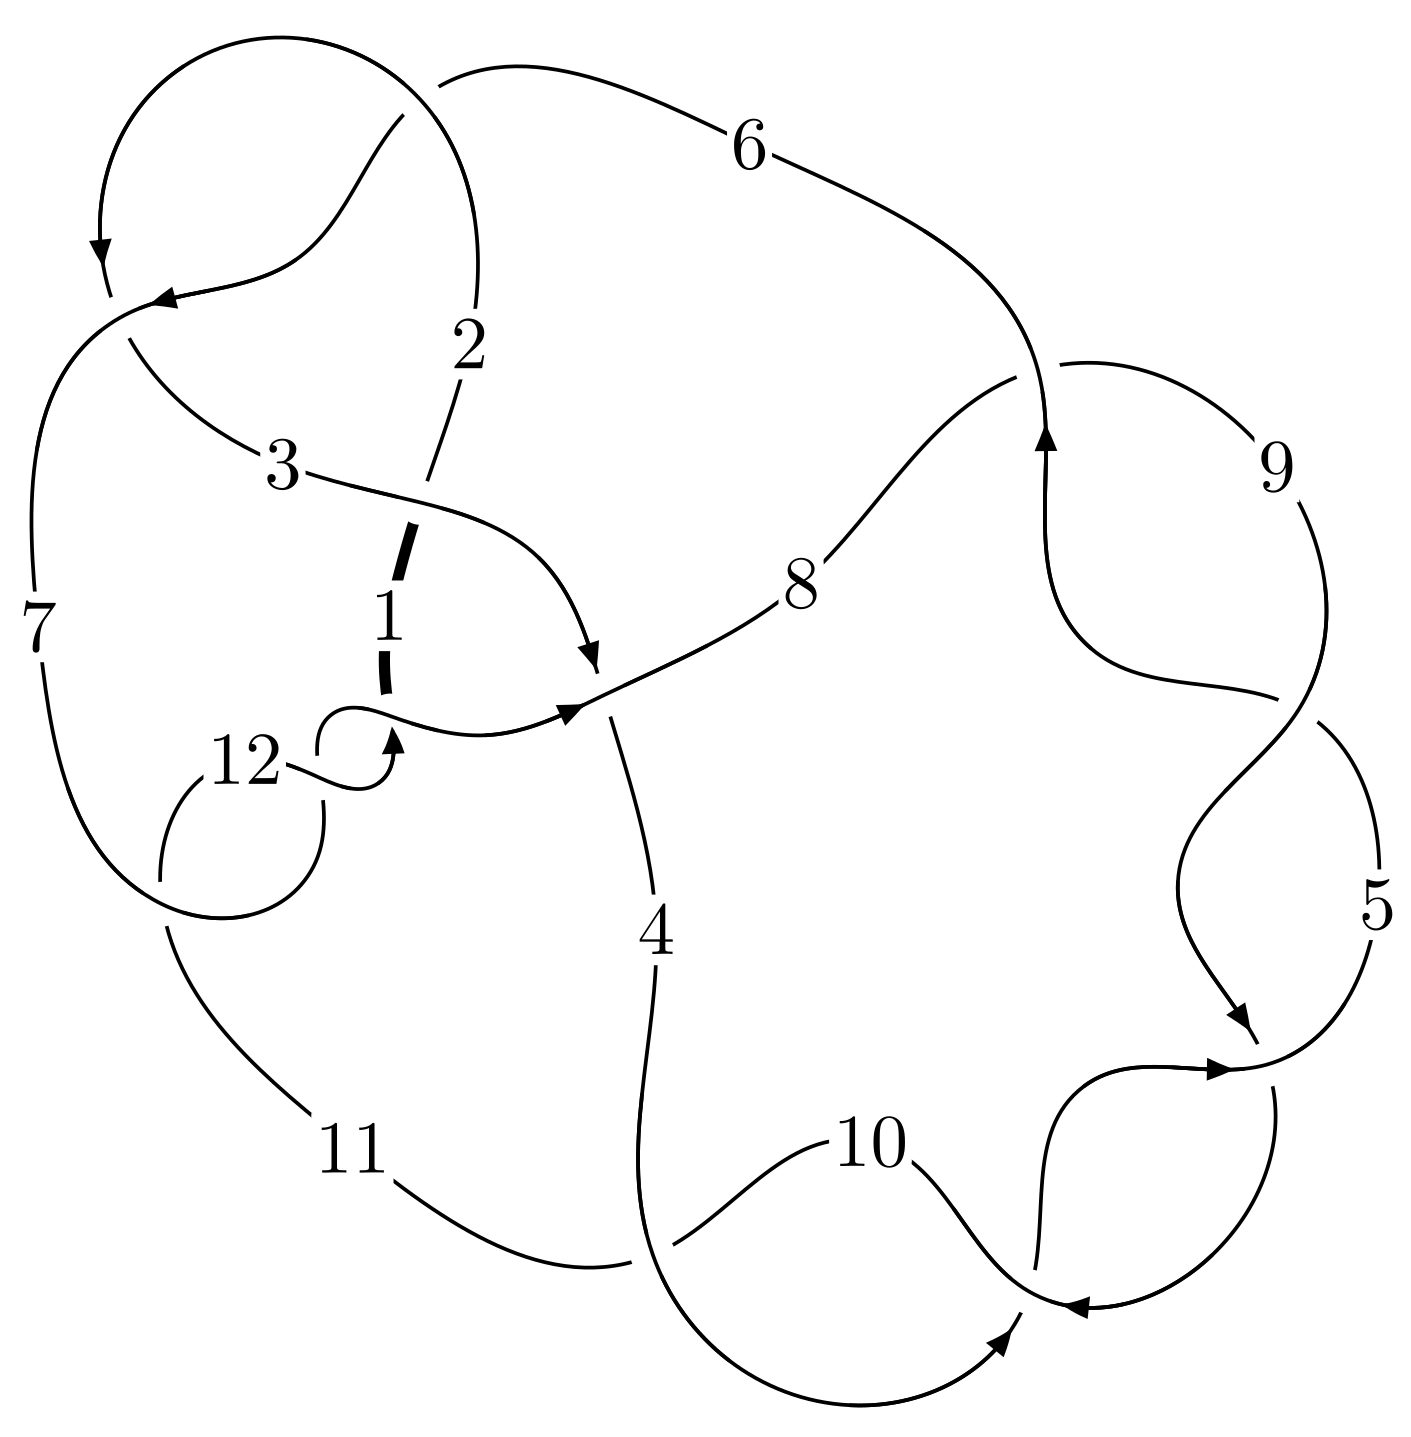
\includegraphics[width=112pt]{../../../GIT/diagram.site/Diagrams/png/2672_12n_0583.png}\\
\ \ \ A knot diagram\footnotemark}&
\allowdisplaybreaks
\textbf{Linearized knot diagam} \\
\cline{2-2}
 &
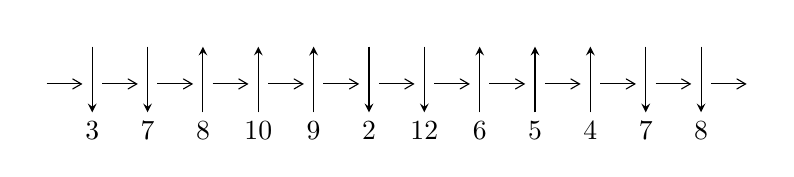
\begin{tikzpicture}[x=20pt, y=17pt]
	% nodes
	\node (C0) at (0, 0) {};
	\node (C1) at (1, 0) {};
	\node (C1U) at (1, +1) {};
	\node (C1D) at (1, -1) {3};

	\node (C2) at (2, 0) {};
	\node (C2U) at (2, +1) {};
	\node (C2D) at (2, -1) {7};

	\node (C3) at (3, 0) {};
	\node (C3U) at (3, +1) {};
	\node (C3D) at (3, -1) {8};

	\node (C4) at (4, 0) {};
	\node (C4U) at (4, +1) {};
	\node (C4D) at (4, -1) {10};

	\node (C5) at (5, 0) {};
	\node (C5U) at (5, +1) {};
	\node (C5D) at (5, -1) {9};

	\node (C6) at (6, 0) {};
	\node (C6U) at (6, +1) {};
	\node (C6D) at (6, -1) {2};

	\node (C7) at (7, 0) {};
	\node (C7U) at (7, +1) {};
	\node (C7D) at (7, -1) {12};

	\node (C8) at (8, 0) {};
	\node (C8U) at (8, +1) {};
	\node (C8D) at (8, -1) {6};

	\node (C9) at (9, 0) {};
	\node (C9U) at (9, +1) {};
	\node (C9D) at (9, -1) {5};

	\node (C10) at (10, 0) {};
	\node (C10U) at (10, +1) {};
	\node (C10D) at (10, -1) {4};

	\node (C11) at (11, 0) {};
	\node (C11U) at (11, +1) {};
	\node (C11D) at (11, -1) {7};

	\node (C12) at (12, 0) {};
	\node (C12U) at (12, +1) {};
	\node (C12D) at (12, -1) {8};
	\node (C13) at (13, 0) {};

	% arrows
	\draw[->,>={angle 60}]
	(C0) edge (C1) (C1) edge (C2) (C2) edge (C3) (C3) edge (C4) (C4) edge (C5) (C5) edge (C6) (C6) edge (C7) (C7) edge (C8) (C8) edge (C9) (C9) edge (C10) (C10) edge (C11) (C11) edge (C12) (C12) edge (C13) ;	\draw[->,>=stealth]
	(C1U) edge (C1D) (C2U) edge (C2D) (C3D) edge (C3U) (C4D) edge (C4U) (C5D) edge (C5U) (C6U) edge (C6D) (C7U) edge (C7D) (C8D) edge (C8U) (C9D) edge (C9U) (C10D) edge (C10U) (C11U) edge (C11D) (C12U) edge (C12D) ;
	\end{tikzpicture} \\
\hhline{~~} \\& 
\textbf{Solving Sequence} \\ \cline{2-2} 
 &
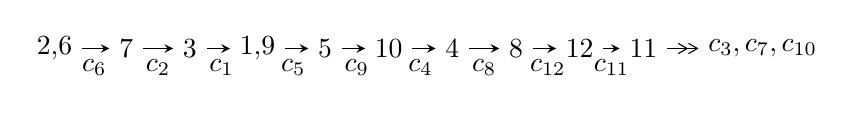
\begin{tikzpicture}[x=23pt, y=7pt]
	% node
	\node (A0) at (-1/8, 0) {2,6};
	\node (A1) at (1, 0) {7};
	\node (A2) at (2, 0) {3};
	\node (A3) at (49/16, 0) {1,9};
	\node (A4) at (33/8, 0) {5};
	\node (A5) at (41/8, 0) {10};
	\node (A6) at (49/8, 0) {4};
	\node (A7) at (57/8, 0) {8};
	\node (A8) at (65/8, 0) {12};
	\node (A9) at (73/8, 0) {11};
	\node (C1) at (1/2, -1) {$c_{6}$};
	\node (C2) at (3/2, -1) {$c_{2}$};
	\node (C3) at (5/2, -1) {$c_{1}$};
	\node (C4) at (29/8, -1) {$c_{5}$};
	\node (C5) at (37/8, -1) {$c_{9}$};
	\node (C6) at (45/8, -1) {$c_{4}$};
	\node (C7) at (53/8, -1) {$c_{8}$};
	\node (C8) at (61/8, -1) {$c_{12}$};
	\node (C9) at (69/8, -1) {$c_{11}$};
	\node (A10) at (11, 0) {$c_{3},c_{7},c_{10}$};

	% edge
	\draw[->,>=stealth]	
	(A0) edge (A1) (A1) edge (A2) (A2) edge (A3) (A3) edge (A4) (A4) edge (A5) (A5) edge (A6) (A6) edge (A7) (A7) edge (A8) (A8) edge (A9) ;
	\draw[->>,>={angle 60}]	
	(A9) edge (A10);
\end{tikzpicture} \\ 

\end{tabular} \\

\footnotetext{
The image of knot diagram is generated by the software ``\textbf{Draw programme}" developed by Andrew Bartholomew(\url{http://www.layer8.co.uk/maths/draw/index.htm\#Running-draw}), where we modified some parts for our purpose(\url{https://github.com/CATsTAILs/LinksPainter}).
}\phantom \\ \newline 
\centering \textbf{Ideals for irreducible components\footnotemark of $X_{\text{par}}$} 
 
\begin{align*}
I^u_{1}&=\langle 
- u^{14}+u^{13}+u^{12}-2 u^{11}-5 u^{10}+6 u^9-6 u^7-7 u^6+8 u^5-2 u^4-4 u^3-7 u^2+4 b+u+1,\\
\phantom{I^u_{1}}&\phantom{= \langle  }- u^{14}+u^{13}+u^{12}-2 u^{11}-5 u^{10}+6 u^9-6 u^7-7 u^6+8 u^5-4 u^4-4 u^3-5 u^2+2 a+u-1,\\
\phantom{I^u_{1}}&\phantom{= \langle  }u^{16}- u^{15}-2 u^{14}+3 u^{13}+6 u^{12}-8 u^{11}-5 u^{10}+12 u^9+7 u^8-14 u^7- u^6+12 u^5+u^4-5 u^3+u+1\rangle \\
I^u_{2}&=\langle 
-1094 u^{19}+352 u^{18}+\cdots+10214 b-24990,\;-4277 u^{19}-4179 u^{18}+\cdots+40856 a+46007,\\
\phantom{I^u_{2}}&\phantom{= \langle  }u^{20}- u^{19}+\cdots+9 u-8\rangle \\
I^u_{3}&=\langle 
2 b- a-1,\;a^2+2 a+13,\;u+1\rangle \\
I^u_{4}&=\langle 
2 b- a-1,\;a^2+2 a+5,\;u-1\rangle \\
I^u_{5}&=\langle 
b,\;a+1,\;u+1\rangle \\
\\
\end{align*}
\raggedright * 5 irreducible components of $\dim_{\mathbb{C}}=0$, with total 41 representations.\\
\footnotetext{All coefficients of polynomials are rational numbers. But the coefficients are sometimes approximated in decimal forms when there is not enough margin.}
\newpage
\renewcommand{\arraystretch}{1}
\centering \section*{I. $I^u_{1}= \langle - u^{14}+u^{13}+\cdots+4 b+1,\;- u^{14}+u^{13}+\cdots+2 a-1,\;u^{16}- u^{15}+\cdots+u+1 \rangle$}
\flushleft \textbf{(i) Arc colorings}\\
\begin{tabular}{m{7pt} m{180pt} m{7pt} m{180pt} }
\flushright $a_{2}=$&$\begin{pmatrix}0\\u\end{pmatrix}$ \\
\flushright $a_{6}=$&$\begin{pmatrix}1\\0\end{pmatrix}$ \\
\flushright $a_{7}=$&$\begin{pmatrix}1\\u^2\end{pmatrix}$ \\
\flushright $a_{3}=$&$\begin{pmatrix}- u\\- u^3+u\end{pmatrix}$ \\
\flushright $a_{1}=$&$\begin{pmatrix}u^3\\u^5- u^3+u\end{pmatrix}$ \\
\flushright $a_{9}=$&$\begin{pmatrix}\frac{1}{2} u^{14}-\frac{1}{2} u^{13}+\cdots-\frac{1}{2} u+\frac{1}{2}\\\frac{1}{4} u^{14}-\frac{1}{4} u^{13}+\cdots-\frac{1}{4} u-\frac{1}{4}\end{pmatrix}$ \\
\flushright $a_{5}=$&$\begin{pmatrix}-\frac{1}{2} u^{15}+\frac{7}{4} u^{14}+\cdots-\frac{7}{4} u-\frac{5}{4}\\-\frac{1}{4} u^{15}+\frac{3}{4} u^{14}+\cdots-\frac{3}{4} u-1\end{pmatrix}$ \\
\flushright $a_{10}=$&$\begin{pmatrix}-\frac{1}{4} u^{15}+\frac{1}{2} u^{14}+\cdots-\frac{1}{2} u-\frac{3}{4}\\\frac{1}{2} u^{13}- u^{12}+\cdots+\frac{1}{2} u^2-\frac{1}{2}\end{pmatrix}$ \\
\flushright $a_{4}=$&$\begin{pmatrix}\frac{5}{4} u^{15}-\frac{3}{2} u^{14}+\cdots-\frac{3}{2} u+\frac{1}{4}\\u^{15}-\frac{5}{4} u^{14}+\cdots-\frac{1}{4} u+\frac{1}{4}\end{pmatrix}$ \\
\flushright $a_{8}=$&$\begin{pmatrix}\frac{1}{4} u^{14}-\frac{1}{4} u^{13}+\cdots-\frac{1}{4} u+\frac{3}{4}\\\frac{1}{4} u^{14}-\frac{1}{4} u^{13}+\cdots-\frac{1}{4} u-\frac{1}{4}\end{pmatrix}$ \\
\flushright $a_{12}=$&$\begin{pmatrix}\frac{1}{4} u^{15}-\frac{1}{4} u^{14}+\cdots-\frac{1}{4} u^2+\frac{3}{4} u\\\frac{1}{4} u^{15}-\frac{1}{4} u^{14}+\cdots-\frac{1}{4} u^2+\frac{3}{4} u\end{pmatrix}$ \\
\flushright $a_{11}=$&$\begin{pmatrix}\frac{1}{4} u^{15}-\frac{1}{4} u^{14}+\cdots-\frac{1}{4} u^2+\frac{7}{4} u\\\frac{1}{4} u^{15}-\frac{1}{4} u^{14}+\cdots-\frac{1}{4} u^2+\frac{3}{4} u\end{pmatrix}$\\&\end{tabular}
\flushleft \textbf{(ii) Obstruction class $= -1$}\\~\\
\flushleft \textbf{(iii) Cusp Shapes $= -\frac{3}{2} u^{15}+\frac{9}{2} u^{14}-\frac{1}{2} u^{13}-10 u^{12}-\frac{1}{2} u^{11}+29 u^{10}-16 u^9-31 u^8+\frac{39}{2} u^7+41 u^6-36 u^5-21 u^4+\frac{53}{2} u^3+\frac{27}{2} u^2-\frac{23}{2} u-6$}\\~\\
\newpage\renewcommand{\arraystretch}{1}
\flushleft \textbf{(iv) u-Polynomials at the component}\newline \\
\begin{tabular}{m{50pt}|m{274pt}}
Crossings & \hspace{64pt}u-Polynomials at each crossing \\
\hline $$\begin{aligned}c_{1}\end{aligned}$$&$\begin{aligned}
&u^{16}+5 u^{15}+\cdots+u+1
\end{aligned}$\\
\hline $$\begin{aligned}c_{2},c_{6},c_{7}\\c_{11},c_{12}\end{aligned}$$&$\begin{aligned}
&u^{16}- u^{15}+\cdots+u+1
\end{aligned}$\\
\hline $$\begin{aligned}c_{3}\end{aligned}$$&$\begin{aligned}
&u^{16}+3 u^{15}+\cdots+146 u+58
\end{aligned}$\\
\hline $$\begin{aligned}c_{4},c_{5},c_{8}\\c_{9},c_{10}\end{aligned}$$&$\begin{aligned}
&u^{16}+3 u^{15}+\cdots+6 u+2
\end{aligned}$\\
\hline
\end{tabular}\\~\\
\newpage\renewcommand{\arraystretch}{1}
\flushleft \textbf{(v) Riley Polynomials at the component}\newline \\
\begin{tabular}{m{50pt}|m{274pt}}
Crossings & \hspace{64pt}Riley Polynomials at each crossing \\
\hline $$\begin{aligned}c_{1}\end{aligned}$$&$\begin{aligned}
&y^{16}+19 y^{15}+\cdots+23 y+1
\end{aligned}$\\
\hline $$\begin{aligned}c_{2},c_{6},c_{7}\\c_{11},c_{12}\end{aligned}$$&$\begin{aligned}
&y^{16}-5 y^{15}+\cdots- y+1
\end{aligned}$\\
\hline $$\begin{aligned}c_{3}\end{aligned}$$&$\begin{aligned}
&y^{16}-3 y^{15}+\cdots+33320 y+3364
\end{aligned}$\\
\hline $$\begin{aligned}c_{4},c_{5},c_{8}\\c_{9},c_{10}\end{aligned}$$&$\begin{aligned}
&y^{16}+21 y^{15}+\cdots+24 y+4
\end{aligned}$\\
\hline
\end{tabular}\\~\\
\newpage\flushleft \textbf{(vi) Complex Volumes and Cusp Shapes}
$$\begin{array}{c|c|c}  
\text{Solutions to }I^u_{1}& \I (\text{vol} + \sqrt{-1}CS) & \text{Cusp shape}\\
 \hline 
\begin{aligned}
u &= \phantom{-}0.652641 + 0.896529 I \\
a &= \phantom{-}0.291031 + 1.146470 I \\
b &= \phantom{-}0.06994 + 1.60049 I\end{aligned}
 & -6.22844 - 0.56003 I & -3.20504 + 2.03342 I \\ \hline\begin{aligned}
u &= \phantom{-}0.652641 - 0.896529 I \\
a &= \phantom{-}0.291031 - 1.146470 I \\
b &= \phantom{-}0.06994 - 1.60049 I\end{aligned}
 & -6.22844 + 0.56003 I & -3.20504 - 2.03342 I \\ \hline\begin{aligned}
u &= -0.806656 + 0.293377 I \\
a &= \phantom{-}0.55147 - 3.56996 I \\
b &= \phantom{-}0.01066 - 1.75439 I\end{aligned}
 & -15.5290 + 1.2535 I & -5.93594 - 5.78561 I \\ \hline\begin{aligned}
u &= -0.806656 - 0.293377 I \\
a &= \phantom{-}0.55147 + 3.56996 I \\
b &= \phantom{-}0.01066 + 1.75439 I\end{aligned}
 & -15.5290 - 1.2535 I & -5.93594 + 5.78561 I \\ \hline\begin{aligned}
u &= -0.863049 + 0.777771 I \\
a &= -0.003821 - 0.394263 I \\
b &= \phantom{-}0.459429 - 0.680536 I\end{aligned}
 & \phantom{-}1.40791 + 2.31178 I & -2.22810 - 1.02238 I \\ \hline\begin{aligned}
u &= -0.863049 - 0.777771 I \\
a &= -0.003821 + 0.394263 I \\
b &= \phantom{-}0.459429 + 0.680536 I\end{aligned}
 & \phantom{-}1.40791 - 2.31178 I & -2.22810 + 1.02238 I \\ \hline\begin{aligned}
u &= \phantom{-}0.699263 + 0.372224 I \\
a &= \phantom{-}0.54747 + 2.11955 I \\
b &= \phantom{-}0.023041 + 1.137640 I\end{aligned}
 & -5.08177 - 1.44001 I & -5.73865 + 4.77821 I \\ \hline\begin{aligned}
u &= \phantom{-}0.699263 - 0.372224 I \\
a &= \phantom{-}0.54747 - 2.11955 I \\
b &= \phantom{-}0.023041 - 1.137640 I\end{aligned}
 & -5.08177 + 1.44001 I & -5.73865 - 4.77821 I \\ \hline\begin{aligned}
u &= \phantom{-}1.000520 + 0.770635 I \\
a &= -0.326142 - 0.537879 I \\
b &= \phantom{-}0.646604 - 0.125765 I\end{aligned}
 & \phantom{-}3.08984 - 6.02737 I & \phantom{-}0.18925 + 5.84414 I \\ \hline\begin{aligned}
u &= \phantom{-}1.000520 - 0.770635 I \\
a &= -0.326142 + 0.537879 I \\
b &= \phantom{-}0.646604 + 0.125765 I\end{aligned}
 & \phantom{-}3.08984 + 6.02737 I & \phantom{-}0.18925 - 5.84414 I\\
 \hline 
 \end{array}$$\newpage$$\begin{array}{c|c|c}  
\text{Solutions to }I^u_{1}& \I (\text{vol} + \sqrt{-1}CS) & \text{Cusp shape}\\
 \hline 
\begin{aligned}
u &= -1.097620 + 0.735783 I \\
a &= -0.99995 + 1.38493 I \\
b &= \phantom{-}0.416151 + 0.956386 I\end{aligned}
 & -0.22230 + 9.61368 I & -4.84554 - 8.00895 I \\ \hline\begin{aligned}
u &= -1.097620 - 0.735783 I \\
a &= -0.99995 - 1.38493 I \\
b &= \phantom{-}0.416151 - 0.956386 I\end{aligned}
 & -0.22230 - 9.61368 I & -4.84554 + 8.00895 I \\ \hline\begin{aligned}
u &= \phantom{-}1.172200 + 0.710728 I \\
a &= -1.65989 - 2.17594 I \\
b &= \phantom{-}0.11516 - 1.70265 I\end{aligned}
 & -9.5315 - 11.7377 I & -6.63835 + 6.61183 I \\ \hline\begin{aligned}
u &= \phantom{-}1.172200 - 0.710728 I \\
a &= -1.65989 + 2.17594 I \\
b &= \phantom{-}0.11516 + 1.70265 I\end{aligned}
 & -9.5315 + 11.7377 I & -6.63835 - 6.61183 I \\ \hline\begin{aligned}
u &= -0.257289 + 0.427551 I \\
a &= \phantom{-}0.599831 - 0.510753 I \\
b &= -0.240981 - 0.391034 I\end{aligned}
 & \phantom{-}0.019028 + 0.937186 I & \phantom{-}0.40237 - 7.45995 I \\ \hline\begin{aligned}
u &= -0.257289 - 0.427551 I \\
a &= \phantom{-}0.599831 + 0.510753 I \\
b &= -0.240981 + 0.391034 I\end{aligned}
 & \phantom{-}0.019028 - 0.937186 I & \phantom{-}0.40237 + 7.45995 I\\
 \hline 
 \end{array}$$\newpage\newpage\renewcommand{\arraystretch}{1}
\centering \section*{II. $I^u_{2}= \langle -1094 u^{19}+352 u^{18}+\cdots+10214 b-24990,\;-4277 u^{19}-4179 u^{18}+\cdots+40856 a+46007,\;u^{20}- u^{19}+\cdots+9 u-8 \rangle$}
\flushleft \textbf{(i) Arc colorings}\\
\begin{tabular}{m{7pt} m{180pt} m{7pt} m{180pt} }
\flushright $a_{2}=$&$\begin{pmatrix}0\\u\end{pmatrix}$ \\
\flushright $a_{6}=$&$\begin{pmatrix}1\\0\end{pmatrix}$ \\
\flushright $a_{7}=$&$\begin{pmatrix}1\\u^2\end{pmatrix}$ \\
\flushright $a_{3}=$&$\begin{pmatrix}- u\\- u^3+u\end{pmatrix}$ \\
\flushright $a_{1}=$&$\begin{pmatrix}u^3\\u^5- u^3+u\end{pmatrix}$ \\
\flushright $a_{9}=$&$\begin{pmatrix}0.104685 u^{19}+0.102286 u^{18}+\cdots-0.766717 u-1.12608\\0.107108 u^{19}-0.0344625 u^{18}+\cdots-0.680537 u+2.44664\end{pmatrix}$ \\
\flushright $a_{5}=$&$\begin{pmatrix}-0.0908312 u^{19}+0.201757 u^{18}+\cdots-0.154714 u-1.48343\\0.265126 u^{19}+0.108479 u^{18}+\cdots-1.49990 u+1.58273\end{pmatrix}$ \\
\flushright $a_{10}=$&$\begin{pmatrix}-0.466370 u^{19}-0.00396515 u^{18}+\cdots+1.09002 u-2.43014\\-0.122968 u^{19}+0.202271 u^{18}+\cdots-0.110828 u-1.64989\end{pmatrix}$ \\
\flushright $a_{4}=$&$\begin{pmatrix}0.305830 u^{19}-0.198722 u^{18}+\cdots-0.0623409 u+2.07194\\-0.154690 u^{19}+0.0378892 u^{18}+\cdots+1.80644 u-1.05639\end{pmatrix}$ \\
\flushright $a_{8}=$&$\begin{pmatrix}-0.00242314 u^{19}+0.136749 u^{18}+\cdots-0.0861807 u-3.57272\\0.107108 u^{19}-0.0344625 u^{18}+\cdots-0.680537 u+2.44664\end{pmatrix}$ \\
\flushright $a_{12}=$&$\begin{pmatrix}0.171505 u^{19}-0.289872 u^{18}+\cdots+4.48857 u+2.09132\\-0.227335 u^{19}+0.238594 u^{18}+\cdots+0.323771 u-1.91326\end{pmatrix}$ \\
\flushright $a_{11}=$&$\begin{pmatrix}\frac{1}{8} u^{19}-\frac{1}{8} u^{18}+\cdots+\frac{19}{8} u+\frac{9}{8}\\-0.0465048 u^{19}+0.164872 u^{18}+\cdots-1.11357 u-0.966321\end{pmatrix}$\\&\end{tabular}
\flushleft \textbf{(ii) Obstruction class $= -1$}\\~\\
\flushleft \textbf{(iii) Cusp Shapes $= \frac{6596}{5107} u^{19}+\frac{828}{5107} u^{18}+\cdots+\frac{15248}{5107} u+\frac{25134}{5107}$}\\~\\
\newpage\renewcommand{\arraystretch}{1}
\flushleft \textbf{(iv) u-Polynomials at the component}\newline \\
\begin{tabular}{m{50pt}|m{274pt}}
Crossings & \hspace{64pt}u-Polynomials at each crossing \\
\hline $$\begin{aligned}c_{1}\end{aligned}$$&$\begin{aligned}
&u^{20}+9 u^{19}+\cdots+385 u+64
\end{aligned}$\\
\hline $$\begin{aligned}c_{2},c_{6},c_{7}\\c_{11},c_{12}\end{aligned}$$&$\begin{aligned}
&u^{20}- u^{19}+\cdots+9 u-8
\end{aligned}$\\
\hline $$\begin{aligned}c_{3}\end{aligned}$$&$\begin{aligned}
&(u^{10}- u^9-5 u^8+4 u^7+8 u^6-3 u^5-5 u^4-2 u^3+3 u^2- u-1)^2
\end{aligned}$\\
\hline $$\begin{aligned}c_{4},c_{5},c_{8}\\c_{9},c_{10}\end{aligned}$$&$\begin{aligned}
&(u^{10}- u^9+7 u^8-6 u^7+16 u^6-11 u^5+13 u^4-6 u^3+3 u^2- u-1)^2
\end{aligned}$\\
\hline
\end{tabular}\\~\\
\newpage\renewcommand{\arraystretch}{1}
\flushleft \textbf{(v) Riley Polynomials at the component}\newline \\
\begin{tabular}{m{50pt}|m{274pt}}
Crossings & \hspace{64pt}Riley Polynomials at each crossing \\
\hline $$\begin{aligned}c_{1}\end{aligned}$$&$\begin{aligned}
&y^{20}+3 y^{19}+\cdots+2431 y+4096
\end{aligned}$\\
\hline $$\begin{aligned}c_{2},c_{6},c_{7}\\c_{11},c_{12}\end{aligned}$$&$\begin{aligned}
&y^{20}-9 y^{19}+\cdots-385 y+64
\end{aligned}$\\
\hline $$\begin{aligned}c_{3}\end{aligned}$$&$\begin{aligned}
&(y^{10}-11 y^9+\cdots-7 y+1)^{2}
\end{aligned}$\\
\hline $$\begin{aligned}c_{4},c_{5},c_{8}\\c_{9},c_{10}\end{aligned}$$&$\begin{aligned}
&(y^{10}+13 y^9+\cdots-7 y+1)^{2}
\end{aligned}$\\
\hline
\end{tabular}\\~\\
\newpage\flushleft \textbf{(vi) Complex Volumes and Cusp Shapes}
$$\begin{array}{c|c|c}  
\text{Solutions to }I^u_{2}& \I (\text{vol} + \sqrt{-1}CS) & \text{Cusp shape}\\
 \hline 
\begin{aligned}
u &= \phantom{-}0.844382 + 0.577422 I \\
a &= -1.82553 - 0.56071 I \\
b &= \phantom{-}0.03425 - 1.67211 I\end{aligned}
 & -14.0102 - 2.2863 I & -7.60221 + 2.91176 I \\ \hline\begin{aligned}
u &= \phantom{-}0.844382 - 0.577422 I \\
a &= -1.82553 + 0.56071 I \\
b &= \phantom{-}0.03425 + 1.67211 I\end{aligned}
 & -14.0102 + 2.2863 I & -7.60221 - 2.91176 I \\ \hline\begin{aligned}
u &= -0.598296 + 0.894963 I \\
a &= \phantom{-}0.237969 + 0.532497 I \\
b &= -0.420834 + 0.842935 I\end{aligned}
 & \phantom{-}1.29172 - 3.55946 I & -2.35774 + 4.06361 I \\ \hline\begin{aligned}
u &= -0.598296 - 0.894963 I \\
a &= \phantom{-}0.237969 - 0.532497 I \\
b &= -0.420834 - 0.842935 I\end{aligned}
 & \phantom{-}1.29172 + 3.55946 I & -2.35774 - 4.06361 I \\ \hline\begin{aligned}
u &= \phantom{-}0.471623 + 0.985477 I \\
a &= \phantom{-}0.169899 - 1.229670 I \\
b &= -0.10787 - 1.66265 I\end{aligned}
 & -7.38803 + 5.55652 I & -4.20810 - 2.88175 I \\ \hline\begin{aligned}
u &= \phantom{-}0.471623 - 0.985477 I \\
a &= \phantom{-}0.169899 + 1.229670 I \\
b &= -0.10787 + 1.66265 I\end{aligned}
 & -7.38803 - 5.55652 I & -4.20810 + 2.88175 I \\ \hline\begin{aligned}
u &= -0.789879 + 0.382389 I \\
a &= -1.61085 - 0.05163 I \\
b &= \phantom{-}0.153406 + 0.833677 I\end{aligned}
 & -5.14913 + 1.60532 I & -7.05654 - 5.03395 I \\ \hline\begin{aligned}
u &= -0.789879 - 0.382389 I \\
a &= -1.61085 + 0.05163 I \\
b &= \phantom{-}0.153406 - 0.833677 I\end{aligned}
 & -5.14913 - 1.60532 I & -7.05654 + 5.03395 I \\ \hline\begin{aligned}
u &= \phantom{-}0.754802 + 0.842126 I \\
a &= \phantom{-}0.394821 + 0.277239 I \\
b &= -0.635590\phantom{ +0.000000I}\end{aligned}
 & \phantom{-}3.84350\phantom{ +0.000000I} & \phantom{-}2.04859 + 0. I\phantom{ +0.000000I} \\ \hline\begin{aligned}
u &= \phantom{-}0.754802 - 0.842126 I \\
a &= \phantom{-}0.394821 - 0.277239 I \\
b &= -0.635590\phantom{ +0.000000I}\end{aligned}
 & \phantom{-}3.84350\phantom{ +0.000000I} & \phantom{-}2.04859 + 0. I\phantom{ +0.000000I}\\
 \hline 
 \end{array}$$\newpage$$\begin{array}{c|c|c}  
\text{Solutions to }I^u_{2}& \I (\text{vol} + \sqrt{-1}CS) & \text{Cusp shape}\\
 \hline 
\begin{aligned}
u &= -1.14103\phantom{ +0.000000I} \\
a &= \phantom{-}0.159161\phantom{ +0.000000I} \\
b &= \phantom{-}0.317683\phantom{ +0.000000I}\end{aligned}
 & -2.68035\phantom{ +0.000000I} & \phantom{-}4.40060\phantom{ +0.000000I} \\ \hline\begin{aligned}
u &= -0.902493 + 0.781683 I \\
a &= \phantom{-}0.910195 - 1.019170 I \\
b &= -0.420834 - 0.842935 I\end{aligned}
 & \phantom{-}1.29172 + 3.55946 I & -2.35774 - 4.06361 I \\ \hline\begin{aligned}
u &= -0.902493 - 0.781683 I \\
a &= \phantom{-}0.910195 + 1.019170 I \\
b &= -0.420834 + 0.842935 I\end{aligned}
 & \phantom{-}1.29172 - 3.55946 I & -2.35774 + 4.06361 I \\ \hline\begin{aligned}
u &= \phantom{-}1.239710 + 0.076961 I \\
a &= \phantom{-}0.06009 + 1.78443 I \\
b &= \phantom{-}0.153406 + 0.833677 I\end{aligned}
 & -5.14913 + 1.60532 I & -7.05654 - 5.03395 I \\ \hline\begin{aligned}
u &= \phantom{-}1.239710 - 0.076961 I \\
a &= \phantom{-}0.06009 - 1.78443 I \\
b &= \phantom{-}0.153406 - 0.833677 I\end{aligned}
 & -5.14913 - 1.60532 I & -7.05654 + 5.03395 I \\ \hline\begin{aligned}
u &= \phantom{-}0.723928\phantom{ +0.000000I} \\
a &= -1.56044\phantom{ +0.000000I} \\
b &= \phantom{-}0.317683\phantom{ +0.000000I}\end{aligned}
 & -2.68035\phantom{ +0.000000I} & \phantom{-}4.40060\phantom{ +0.000000I} \\ \hline\begin{aligned}
u &= \phantom{-}1.043190 + 0.765280 I \\
a &= \phantom{-}1.48424 + 1.76241 I \\
b &= -0.10787 + 1.66265 I\end{aligned}
 & -7.38803 - 5.55652 I & -4.20810 + 2.88175 I \\ \hline\begin{aligned}
u &= \phantom{-}1.043190 - 0.765280 I \\
a &= \phantom{-}1.48424 - 1.76241 I \\
b &= -0.10787 - 1.66265 I\end{aligned}
 & -7.38803 + 5.55652 I & -4.20810 - 2.88175 I \\ \hline\begin{aligned}
u &= -1.354480 + 0.103519 I \\
a &= \phantom{-}0.06730 - 3.11843 I \\
b &= \phantom{-}0.03425 - 1.67211 I\end{aligned}
 & -14.0102 - 2.2863 I & -7.60221 + 2.91176 I \\ \hline\begin{aligned}
u &= -1.354480 - 0.103519 I \\
a &= \phantom{-}0.06730 + 3.11843 I \\
b &= \phantom{-}0.03425 + 1.67211 I\end{aligned}
 & -14.0102 + 2.2863 I & -7.60221 - 2.91176 I\\
 \hline 
 \end{array}$$\newpage\newpage\renewcommand{\arraystretch}{1}
\centering \section*{III. $I^u_{3}= \langle 2 b- a-1,\;a^2+2 a+13,\;u+1 \rangle$}
\flushleft \textbf{(i) Arc colorings}\\
\begin{tabular}{m{7pt} m{180pt} m{7pt} m{180pt} }
\flushright $a_{2}=$&$\begin{pmatrix}0\\-1\end{pmatrix}$ \\
\flushright $a_{6}=$&$\begin{pmatrix}1\\0\end{pmatrix}$ \\
\flushright $a_{7}=$&$\begin{pmatrix}1\\1\end{pmatrix}$ \\
\flushright $a_{3}=$&$\begin{pmatrix}1\\0\end{pmatrix}$ \\
\flushright $a_{1}=$&$\begin{pmatrix}-1\\-1\end{pmatrix}$ \\
\flushright $a_{9}=$&$\begin{pmatrix}a\\\frac{1}{2} a+\frac{1}{2}\end{pmatrix}$ \\
\flushright $a_{5}=$&$\begin{pmatrix}-\frac{1}{2} a-\frac{11}{2}\\-3\end{pmatrix}$ \\
\flushright $a_{10}=$&$\begin{pmatrix}-\frac{3}{2} a+\frac{1}{2}\\- a-1\end{pmatrix}$ \\
\flushright $a_{4}=$&$\begin{pmatrix}\frac{1}{2} a+\frac{9}{2}\\3\end{pmatrix}$ \\
\flushright $a_{8}=$&$\begin{pmatrix}\frac{1}{2} a-\frac{1}{2}\\\frac{1}{2} a+\frac{1}{2}\end{pmatrix}$ \\
\flushright $a_{12}=$&$\begin{pmatrix}\frac{1}{2} a-\frac{3}{2}\\\frac{1}{2} a-\frac{1}{2}\end{pmatrix}$ \\
\flushright $a_{11}=$&$\begin{pmatrix}\frac{1}{2} a-\frac{1}{2}\\\frac{1}{2} a+\frac{1}{2}\end{pmatrix}$\\&\end{tabular}
\flushleft \textbf{(ii) Obstruction class $= 1$}\\~\\
\flushleft \textbf{(iii) Cusp Shapes $= -12$}\\~\\
\newpage\renewcommand{\arraystretch}{1}
\flushleft \textbf{(iv) u-Polynomials at the component}\newline \\
\begin{tabular}{m{50pt}|m{274pt}}
Crossings & \hspace{64pt}u-Polynomials at each crossing \\
\hline $$\begin{aligned}c_{1},c_{2},c_{7}\end{aligned}$$&$\begin{aligned}
&(u-1)^2
\end{aligned}$\\
\hline $$\begin{aligned}c_{3},c_{4},c_{5}\\c_{8},c_{9},c_{10}\end{aligned}$$&$\begin{aligned}
&u^2+3
\end{aligned}$\\
\hline $$\begin{aligned}c_{6},c_{11},c_{12}\end{aligned}$$&$\begin{aligned}
&(u+1)^2
\end{aligned}$\\
\hline
\end{tabular}\\~\\
\newpage\renewcommand{\arraystretch}{1}
\flushleft \textbf{(v) Riley Polynomials at the component}\newline \\
\begin{tabular}{m{50pt}|m{274pt}}
Crossings & \hspace{64pt}Riley Polynomials at each crossing \\
\hline $$\begin{aligned}c_{1},c_{2},c_{6}\\c_{7},c_{11},c_{12}\end{aligned}$$&$\begin{aligned}
&(y-1)^2
\end{aligned}$\\
\hline $$\begin{aligned}c_{3},c_{4},c_{5}\\c_{8},c_{9},c_{10}\end{aligned}$$&$\begin{aligned}
&(y+3)^2
\end{aligned}$\\
\hline
\end{tabular}\\~\\
\newpage\flushleft \textbf{(vi) Complex Volumes and Cusp Shapes}
$$\begin{array}{c|c|c}  
\text{Solutions to }I^u_{3}& \I (\text{vol} + \sqrt{-1}CS) & \text{Cusp shape}\\
 \hline 
\begin{aligned}
u &= -1.00000\phantom{ +0.000000I} \\
a &= -1.00000 + 3.46410 I \\
b &= \phantom{-0.000000 -}1.73205 I\end{aligned}
 & -16.4493\phantom{ +0.000000I} & -12.0000\phantom{ +0.000000I} \\ \hline\begin{aligned}
u &= -1.00000\phantom{ +0.000000I} \\
a &= -1.00000 - 3.46410 I \\
b &= \phantom{-0.000000 } -1.73205 I\end{aligned}
 & -16.4493\phantom{ +0.000000I} & -12.0000\phantom{ +0.000000I}\\
 \hline 
 \end{array}$$\newpage\newpage\renewcommand{\arraystretch}{1}
\centering \section*{IV. $I^u_{4}= \langle 2 b- a-1,\;a^2+2 a+5,\;u-1 \rangle$}
\flushleft \textbf{(i) Arc colorings}\\
\begin{tabular}{m{7pt} m{180pt} m{7pt} m{180pt} }
\flushright $a_{2}=$&$\begin{pmatrix}0\\1\end{pmatrix}$ \\
\flushright $a_{6}=$&$\begin{pmatrix}1\\0\end{pmatrix}$ \\
\flushright $a_{7}=$&$\begin{pmatrix}1\\1\end{pmatrix}$ \\
\flushright $a_{3}=$&$\begin{pmatrix}-1\\0\end{pmatrix}$ \\
\flushright $a_{1}=$&$\begin{pmatrix}1\\1\end{pmatrix}$ \\
\flushright $a_{9}=$&$\begin{pmatrix}a\\\frac{1}{2} a+\frac{1}{2}\end{pmatrix}$ \\
\flushright $a_{5}=$&$\begin{pmatrix}-\frac{1}{2} a-\frac{3}{2}\\-1\end{pmatrix}$ \\
\flushright $a_{10}=$&$\begin{pmatrix}\frac{1}{2} a+\frac{1}{2}\\0\end{pmatrix}$ \\
\flushright $a_{4}=$&$\begin{pmatrix}-\frac{1}{2} a-\frac{5}{2}\\-1\end{pmatrix}$ \\
\flushright $a_{8}=$&$\begin{pmatrix}\frac{1}{2} a-\frac{1}{2}\\\frac{1}{2} a+\frac{1}{2}\end{pmatrix}$ \\
\flushright $a_{12}=$&$\begin{pmatrix}-\frac{1}{2} a+\frac{3}{2}\\-\frac{1}{2} a+\frac{1}{2}\end{pmatrix}$ \\
\flushright $a_{11}=$&$\begin{pmatrix}-\frac{1}{2} a+\frac{1}{2}\\-\frac{1}{2} a-\frac{1}{2}\end{pmatrix}$\\&\end{tabular}
\flushleft \textbf{(ii) Obstruction class $= 1$}\\~\\
\flushleft \textbf{(iii) Cusp Shapes $= -12$}\\~\\
\newpage\renewcommand{\arraystretch}{1}
\flushleft \textbf{(iv) u-Polynomials at the component}\newline \\
\begin{tabular}{m{50pt}|m{274pt}}
Crossings & \hspace{64pt}u-Polynomials at each crossing \\
\hline $$\begin{aligned}c_{1},c_{6},c_{11}\\c_{12}\end{aligned}$$&$\begin{aligned}
&(u-1)^2
\end{aligned}$\\
\hline $$\begin{aligned}c_{2},c_{7}\end{aligned}$$&$\begin{aligned}
&(u+1)^2
\end{aligned}$\\
\hline $$\begin{aligned}c_{3},c_{4},c_{5}\\c_{8},c_{9},c_{10}\end{aligned}$$&$\begin{aligned}
&u^2+1
\end{aligned}$\\
\hline
\end{tabular}\\~\\
\newpage\renewcommand{\arraystretch}{1}
\flushleft \textbf{(v) Riley Polynomials at the component}\newline \\
\begin{tabular}{m{50pt}|m{274pt}}
Crossings & \hspace{64pt}Riley Polynomials at each crossing \\
\hline $$\begin{aligned}c_{1},c_{2},c_{6}\\c_{7},c_{11},c_{12}\end{aligned}$$&$\begin{aligned}
&(y-1)^2
\end{aligned}$\\
\hline $$\begin{aligned}c_{3},c_{4},c_{5}\\c_{8},c_{9},c_{10}\end{aligned}$$&$\begin{aligned}
&(y+1)^2
\end{aligned}$\\
\hline
\end{tabular}\\~\\
\newpage\flushleft \textbf{(vi) Complex Volumes and Cusp Shapes}
$$\begin{array}{c|c|c}  
\text{Solutions to }I^u_{4}& \I (\text{vol} + \sqrt{-1}CS) & \text{Cusp shape}\\
 \hline 
\begin{aligned}
u &= \phantom{-}1.00000\phantom{ +0.000000I} \\
a &= -1.00000 + 2.00000 I \\
b &= \phantom{-0.000000 -}1.000000 I\end{aligned}
 & -6.57974\phantom{ +0.000000I} & -12.0000\phantom{ +0.000000I} \\ \hline\begin{aligned}
u &= \phantom{-}1.00000\phantom{ +0.000000I} \\
a &= -1.00000 - 2.00000 I \\
b &= \phantom{-0.000000 } -1.000000 I\end{aligned}
 & -6.57974\phantom{ +0.000000I} & -12.0000\phantom{ +0.000000I}\\
 \hline 
 \end{array}$$\newpage\newpage\renewcommand{\arraystretch}{1}
\centering \section*{V. $I^u_{5}= \langle b,\;a+1,\;u+1 \rangle$}
\flushleft \textbf{(i) Arc colorings}\\
\begin{tabular}{m{7pt} m{180pt} m{7pt} m{180pt} }
\flushright $a_{2}=$&$\begin{pmatrix}0\\-1\end{pmatrix}$ \\
\flushright $a_{6}=$&$\begin{pmatrix}1\\0\end{pmatrix}$ \\
\flushright $a_{7}=$&$\begin{pmatrix}1\\1\end{pmatrix}$ \\
\flushright $a_{3}=$&$\begin{pmatrix}1\\0\end{pmatrix}$ \\
\flushright $a_{1}=$&$\begin{pmatrix}-1\\-1\end{pmatrix}$ \\
\flushright $a_{9}=$&$\begin{pmatrix}-1\\0\end{pmatrix}$ \\
\flushright $a_{5}=$&$\begin{pmatrix}1\\0\end{pmatrix}$ \\
\flushright $a_{10}=$&$\begin{pmatrix}-1\\0\end{pmatrix}$ \\
\flushright $a_{4}=$&$\begin{pmatrix}1\\0\end{pmatrix}$ \\
\flushright $a_{8}=$&$\begin{pmatrix}-1\\0\end{pmatrix}$ \\
\flushright $a_{12}=$&$\begin{pmatrix}-2\\-1\end{pmatrix}$ \\
\flushright $a_{11}=$&$\begin{pmatrix}-1\\0\end{pmatrix}$\\&\end{tabular}
\flushleft \textbf{(ii) Obstruction class $= 1$}\\~\\
\flushleft \textbf{(iii) Cusp Shapes $= -12$}\\~\\
\newpage\renewcommand{\arraystretch}{1}
\flushleft \textbf{(iv) u-Polynomials at the component}\newline \\
\begin{tabular}{m{50pt}|m{274pt}}
Crossings & \hspace{64pt}u-Polynomials at each crossing \\
\hline $$\begin{aligned}c_{1},c_{2},c_{7}\end{aligned}$$&$\begin{aligned}
&u-1
\end{aligned}$\\
\hline $$\begin{aligned}c_{3},c_{4},c_{5}\\c_{8},c_{9},c_{10}\end{aligned}$$&$\begin{aligned}
&u
\end{aligned}$\\
\hline $$\begin{aligned}c_{6},c_{11},c_{12}\end{aligned}$$&$\begin{aligned}
&u+1
\end{aligned}$\\
\hline
\end{tabular}\\~\\
\newpage\renewcommand{\arraystretch}{1}
\flushleft \textbf{(v) Riley Polynomials at the component}\newline \\
\begin{tabular}{m{50pt}|m{274pt}}
Crossings & \hspace{64pt}Riley Polynomials at each crossing \\
\hline $$\begin{aligned}c_{1},c_{2},c_{6}\\c_{7},c_{11},c_{12}\end{aligned}$$&$\begin{aligned}
&y-1
\end{aligned}$\\
\hline $$\begin{aligned}c_{3},c_{4},c_{5}\\c_{8},c_{9},c_{10}\end{aligned}$$&$\begin{aligned}
&y
\end{aligned}$\\
\hline
\end{tabular}\\~\\
\newpage\flushleft \textbf{(vi) Complex Volumes and Cusp Shapes}
$$\begin{array}{c|c|c}  
\text{Solutions to }I^u_{5}& \I (\text{vol} + \sqrt{-1}CS) & \text{Cusp shape}\\
 \hline 
\begin{aligned}
u &= -1.00000\phantom{ +0.000000I} \\
a &= -1.00000\phantom{ +0.000000I} \\
b &= \phantom{-0.000000 } 0\end{aligned}
 & -3.28987\phantom{ +0.000000I} & -12.0000\phantom{ +0.000000I}\\
 \hline 
 \end{array}$$\newpage
\newpage\renewcommand{\arraystretch}{1}
\centering \section*{ VI. u-Polynomials}
\begin{tabular}{m{50pt}|m{274pt}}
Crossings & \hspace{64pt}u-Polynomials at each crossing \\
\hline $$\begin{aligned}c_{1}\end{aligned}$$&$\begin{aligned}
&((u-1)^5)(u^{16}+5 u^{15}+\cdots+u+1)(u^{20}+9 u^{19}+\cdots+385 u+64)
\end{aligned}$\\
\hline $$\begin{aligned}c_{2},c_{7}\end{aligned}$$&$\begin{aligned}
&((u-1)^3)(u+1)^2(u^{16}- u^{15}+\cdots+u+1)(u^{20}- u^{19}+\cdots+9 u-8)
\end{aligned}$\\
\hline $$\begin{aligned}c_{3}\end{aligned}$$&$\begin{aligned}
&u(u^2+1)(u^2+3)\\
&\cdot(u^{10}- u^9-5 u^8+4 u^7+8 u^6-3 u^5-5 u^4-2 u^3+3 u^2- u-1)^2\\
&\cdot(u^{16}+3 u^{15}+\cdots+146 u+58)
\end{aligned}$\\
\hline $$\begin{aligned}c_{4},c_{5},c_{8}\\c_{9},c_{10}\end{aligned}$$&$\begin{aligned}
&u(u^2+1)(u^2+3)\\
&\cdot(u^{10}- u^9+7 u^8-6 u^7+16 u^6-11 u^5+13 u^4-6 u^3+3 u^2- u-1)^2\\
&\cdot(u^{16}+3 u^{15}+\cdots+6 u+2)
\end{aligned}$\\
\hline $$\begin{aligned}c_{6},c_{11},c_{12}\end{aligned}$$&$\begin{aligned}
&((u-1)^2)(u+1)^3(u^{16}- u^{15}+\cdots+u+1)(u^{20}- u^{19}+\cdots+9 u-8)
\end{aligned}$\\
\hline
\end{tabular}\newpage\renewcommand{\arraystretch}{1}
\centering \section*{ VII. Riley Polynomials}
\begin{tabular}{m{50pt}|m{274pt}}
Crossings & \hspace{64pt}Riley Polynomials at each crossing \\
\hline $$\begin{aligned}c_{1}\end{aligned}$$&$\begin{aligned}
&((y-1)^5)(y^{16}+19 y^{15}+\cdots+23 y+1)\\
&\cdot(y^{20}+3 y^{19}+\cdots+2431 y+4096)
\end{aligned}$\\
\hline $$\begin{aligned}c_{2},c_{6},c_{7}\\c_{11},c_{12}\end{aligned}$$&$\begin{aligned}
&((y-1)^5)(y^{16}-5 y^{15}+\cdots- y+1)(y^{20}-9 y^{19}+\cdots-385 y+64)
\end{aligned}$\\
\hline $$\begin{aligned}c_{3}\end{aligned}$$&$\begin{aligned}
&y(y+1)^2(y+3)^2(y^{10}-11 y^{9}+\cdots-7 y+1)^{2}\\
&\cdot(y^{16}-3 y^{15}+\cdots+33320 y+3364)
\end{aligned}$\\
\hline $$\begin{aligned}c_{4},c_{5},c_{8}\\c_{9},c_{10}\end{aligned}$$&$\begin{aligned}
&y(y+1)^2(y+3)^2(y^{10}+13 y^{9}+\cdots-7 y+1)^{2}\\
&\cdot(y^{16}+21 y^{15}+\cdots+24 y+4)
\end{aligned}$\\
\hline
\end{tabular}
\vskip 2pc
\end{document}